\documentclass[11pt, oneside]{article}   	% use "amsart" instead of "article" for AMSLaTeX format
\usepackage{geometry}                		% See geometry.pdf to learn the layout options. There are lots.
\geometry{a4paper}                   		% ... or a4paper or a5paper or ... 
%\geometry{landscape}				% Activate for for rotated page geometry
\usepackage[parfill]{parskip}			% Activate to begin paragraphs with an empty line rather than an indent
\usepackage{graphicx}				% Use pdf, png, jpg, or eps§ with pdflatex; use eps in DVI mode

\usepackage{amssymb}
\usepackage{mhchem}
\usepackage{gensymb}
\usepackage{textcomp}
\usepackage{braket}
\usepackage{amsmath}
\usepackage{multirow}

\title{600.438 Computational Genomics \\ Age-related Changes in Gene Expression in \\ Humans and Link to Disease}
\author{Sachi Sanghavi}

\begin{document}
\maketitle

\section{Motivation}

Aging is a universal biological process; and is known to be a major risk factor in diseases like type-2 diabetes, cancer, Alzheimer's disease, and more. However, the underlying molecular mechanisms of aging are still not well understood. This leaves the question ``Is aging genetically programmed?'' open for debate. Studying the association between aging and gene expression might give us some insights which could lead to novel treatments for treating age-related diseases.

We present a study of aging -- gene expression association in humans in subcutaneous adipose tissue\footnote{The original plan was to use two tissue samples: subcutaneous adipose tissue and whole blood tissue, but due to time restrictions, only the former was used. However, note that the process is same for all.} and its link to disease.

\section{Background}

The study is based off of Yang \emph{et al.} (2015). Though the initial aim was to follow the study as close as possible and try and replicate the results, along the way,---both due to non-clarity [on our side] and time restrictions---we carried out only a subset of the experimental tasks from the study.

An important point to note is that our study made use of \emph{more} samples for the same tissues. So, it is possible we might have better statistics, but the benefits are not apparent since our methods are not exactly the same as Yang \emph{et al.} (2015).

\section{Aims and Methods}

\begin{enumerate}
\item Find age -- gene expression association and report it for top 100 genes for human subcutaneous adipose tissue
	\begin{itemize}
	\item Correct for confounding factors in gene expression data using PCA and factor analysis \emph{\`{a} la} Pickrell \emph{et al.} (2010)---correct for gender, top 3 genotype PCs, and top 5 genotype PCs (those not significantly correlated with age, that is p-value $>0.05$).
	\item Use linear regression to find aging genes; conduct false discovery rate adjustment (FDR) on p-values using Benjamini Hochberg method.
	\item Remove 20\% low expressed aging genes\footnote{Yang \emph{et al.} (2015) also made use of bootstrapping and permutation to control for false positives. Since we only used one tissue, adipose, and since it did not show any permutation effects in Yang \emph{et al.} (2015), we decided to take the short-cut approach.}.
	\end{itemize}
\item Functional annotation of aging genes [up- and down-regulated separately]
	\begin{itemize}
	\item Use David tools.
	\end{itemize}
\item Tissue specific link between aging genes and complex disease genes.
	\begin{itemize}
	\item Disease gene data compiled from NIH GWAS\footnote{Yang \emph{et al.} (2015) compiled disease gene data from NIH GWAS and OHIM using clustering.}.
	\item Fisher's test for aging -- diseases genes link.
	\end{itemize}
\item Compare results with Yang \emph{et al.} (2015).
\end{enumerate}

\begin{figure}[!ht]
    \centering
    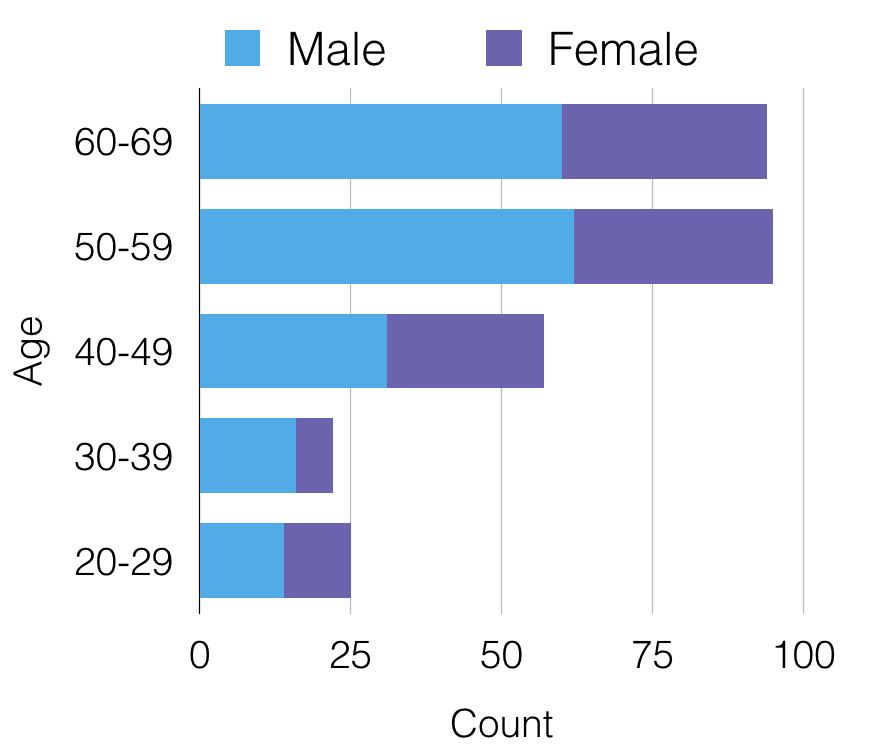
\includegraphics[width=0.50\textwidth]{stats}
    \caption{\textbf{Age distribution of adipose tissue donors.}}
    \label{fig:stats}
\end{figure}

\section{Data}

Gene expression data is taken from GTEx project v6, along with a covariates matrix (containing gender, top 3 genotypes PCs, platform, and some PEER covariates). GTEx has available gene expression levels for 27,182 genes from human subcutaneous adipose tissue with a sample size of 298. See figure \ref{fig:stats} for age and gender distribution of tissue donors.

GTEx and GWAS accessed on April 27, 2016.

\section{Results}

\subsection*{Correcting for confounding factors based on PCA}

In studies using RNA-seq data, correction for technical confounders (like batch effects, sample processing, etc.) and biological variables (like gender, ancestry, etc.) is an important step to get true underlying associations and other signal detections.

Yang \emph{et al.} (2015) follow the PCA based approach used by Pickrell \emph{et al.} (2010), to correct for gender, top 3 genotype PCs and gene expression PCs that do no significantly (p-value) correlate with age (this comes out to be 5 gene expression PCs) (since, in our case, age can be one of the top gene expression PCs).

The approach is simple:
\begin{enumerate}
\item We call \texttt{dudi.pca} function from \texttt{ade4} package in R on our gene expression levels.
\item For each individual, we extract their loadings or PCs [for top 5 PCs, following Yang \emph{et al.} (2015)].
\item Then, for each gene, we perform linear regression using model
$$ \hat{H}_0: Y_{ij} = \beta_{j} + \delta_{j} \text{Sex}_{i} + \sum_{k=1}^{3} \mu_{jk} \text{Genotype}_{ik} + \sum_{k=1}^{5} \alpha_{jk} \text{PC}_{ik} + \epsilon_{ij} $$
where $ Y_{ij} $ is the expression level of gene $ j $ in sample $ i $, $ \text{Sex}_{i} $ denotes sex of sample $ i $, $ \text{Genotype}_{ik} (1 \leq k \leq 3) $ denotes \emph{k}-th genotype PC value for the \emph{i}-th sample, and $ \text{PC}_{ik} (1 \leq k \leq 5) $ denotes \emph{k}-th gene expression PC value.
\item Now, we use the residuals found in the previous step as our new gene expression matrix; that is
$$ Y_{ij}^{\text{new}} = Y_{ij} - \sum_{k=1}^{5} \alpha_{jk} \text{PC}_{ik} $$
\end{enumerate}


\subsection*{Linear regression for aging gene detection}

With the new gene expression matrix $ Y_{ij}^{\text{new}} $ found in the previous section, we perform linear regression to detect aging genes

$$ \hat{H}_1: Y_{ij}^{\text{new}} = \beta_{j} + \gamma_{j} \text{Age}_{i} + \delta_{j} \text{Sex}_{i} + \sum_{k=1}^{3} \mu_{jk} \text{Genotype}_{ik} + \sum_{k=1}^{5} \alpha_{jk} \text{PC}_{ik} + \epsilon_{ij} $$

Just as in Yang \emph{et al.} (2015), if $ \gamma_{j} $ deviated significantly (p-value $<$ 0.05) from 0, gene $ j $ was considered to be age-associated. Gene $ j $ was up-regulated if $ \gamma_{j} > 0 $, and down-regulated if $ \gamma_{j} < 0 $. At this point, we had 3345 aging genes.

False discovery rate (FDR) adjustment was done on p-values using Benjamini Hochberg method (threshold of 0.05). At this point, we were left with 242 aging genes.

Then, we removed 20\% low expressed aging genes: (i) we ranked the aging genes based on their expression levels in descending order, (ii) we calculated the mean expression levels of the top 25\% samples, and ranked the samples according to mean expression value in descending order, and then (iii) we removed bottom 20\% aging genes.

Our final count of aging genes was 194\footnote{\emph{\textbf{N.B.}} From my understanding, Pickrell \emph{et al.} (2010) makes use of PCA \emph{and} factor analysis to remove top \emph{N} gene expression PCs. To do this, generally you loop steps (i)-(iv) and linear regression if $\hat{H}_1 > \hat{H}_0$, until you finally have residual matrix with top $i$ gene expression PCs removed, checked by $\hat{H}_i > \hat{H}_{i-1}$ and $\hat{H}_i > \hat{H}_{i+1}$. We then use whatever residual matrix we have at this point as our new gene expression matrix. However, Yang \emph{et al.} (2015) never described this, so we just ended up using top \emph{5} gene expression PCs like they did. From the scree plots, you see that 5 PCs don't really capture much variance in the data, and this confused me as well [in that, I'm not sure if using 5 was the best decision].}.

For a strongly expressed aging gene, \texttt{ENSG00000048540.10}, we plotted Residuals vs Fitted, Q-Q, Scale-Location, and Residuals vs Leverage plots.

\begin{table}[b]
\centering
\begin{tabular}{|c|c|c|c|c|c|c|c|c|}
\hline
\multirow{3}{*}{\textbf{Tissues}} & \multicolumn{4}{c|}{\textbf{Our Results}}                                              & \multicolumn{4}{c|}{\textbf{Yang et al. (2015)}}                                       \\ \cline{2-9} 
                                  & \multirow{2}{*}{\textbf{Sample Size}} & \multicolumn{3}{c|}{\textbf{Aging gene}}       & \multirow{2}{*}{\textbf{Sample Size}} & \multicolumn{3}{c|}{\textbf{Aging gene}}       \\ \cline{3-5} \cline{7-9} 
                                  &                                       & \textbf{Up} & \textbf{Down} & \textbf{Overall} &                                       & \textbf{Up} & \textbf{Down} & \textbf{Overall} \\ \hline
\multicolumn{1}{|l|}{Adipose}     & 298                                   & 127         & 67            & 194              & 94                                    & 652         & 482           & 1134             \\ \hline
\end{tabular}
\caption{\textbf{Number of age-associated genes in human adipose tissue.}}
\label{table:aging-genes}
\end{table}

\subsection*{Functional annotation of aging genes}

We used David tools for functional annotation of the aging genes, providing a list of Ensembl IDs as the input. The program could only annotate 162 out of the 194 aging genes. We only considered diseases with at lest 5 genes, and set the age-disease p-value threshold at 0.05.

See the text files under \texttt{davidtools} folder for data.

\section{Additional notes}

As it was suggested in the feedback form, testing for \texttt{age x gender} association on gene expression levels would be interesting, though we couldn't get around to it. Also, clustering on aging genes' expression levels could be helpful too, but David tools already provides the functionality (plus, we don't have a good enough number of aging genes to get sensible results). 

A heatmap for top age-associated genes was plotted, but we did not observe any `young' and `old' clustering. It's possibly because we don't have a good enough number of aging genes (also, it is highly likely our dendrogram might not have been used correctly).


\end{document}